\chapter{Running a test}\label{chap::run}
Once a test has been configured or opened from an existing file, you will be taken to the 'Test Menu', and you can begin running it. On the screen shown below in Figure \ref{run::testingMenu}, you can begin the test with new subject by clicking \emph{New Subject}, or continue with an existing one that has not yet completed all sessions by clicking \emph{Continue}. 

\begin{figure}[ht]
	\centering
	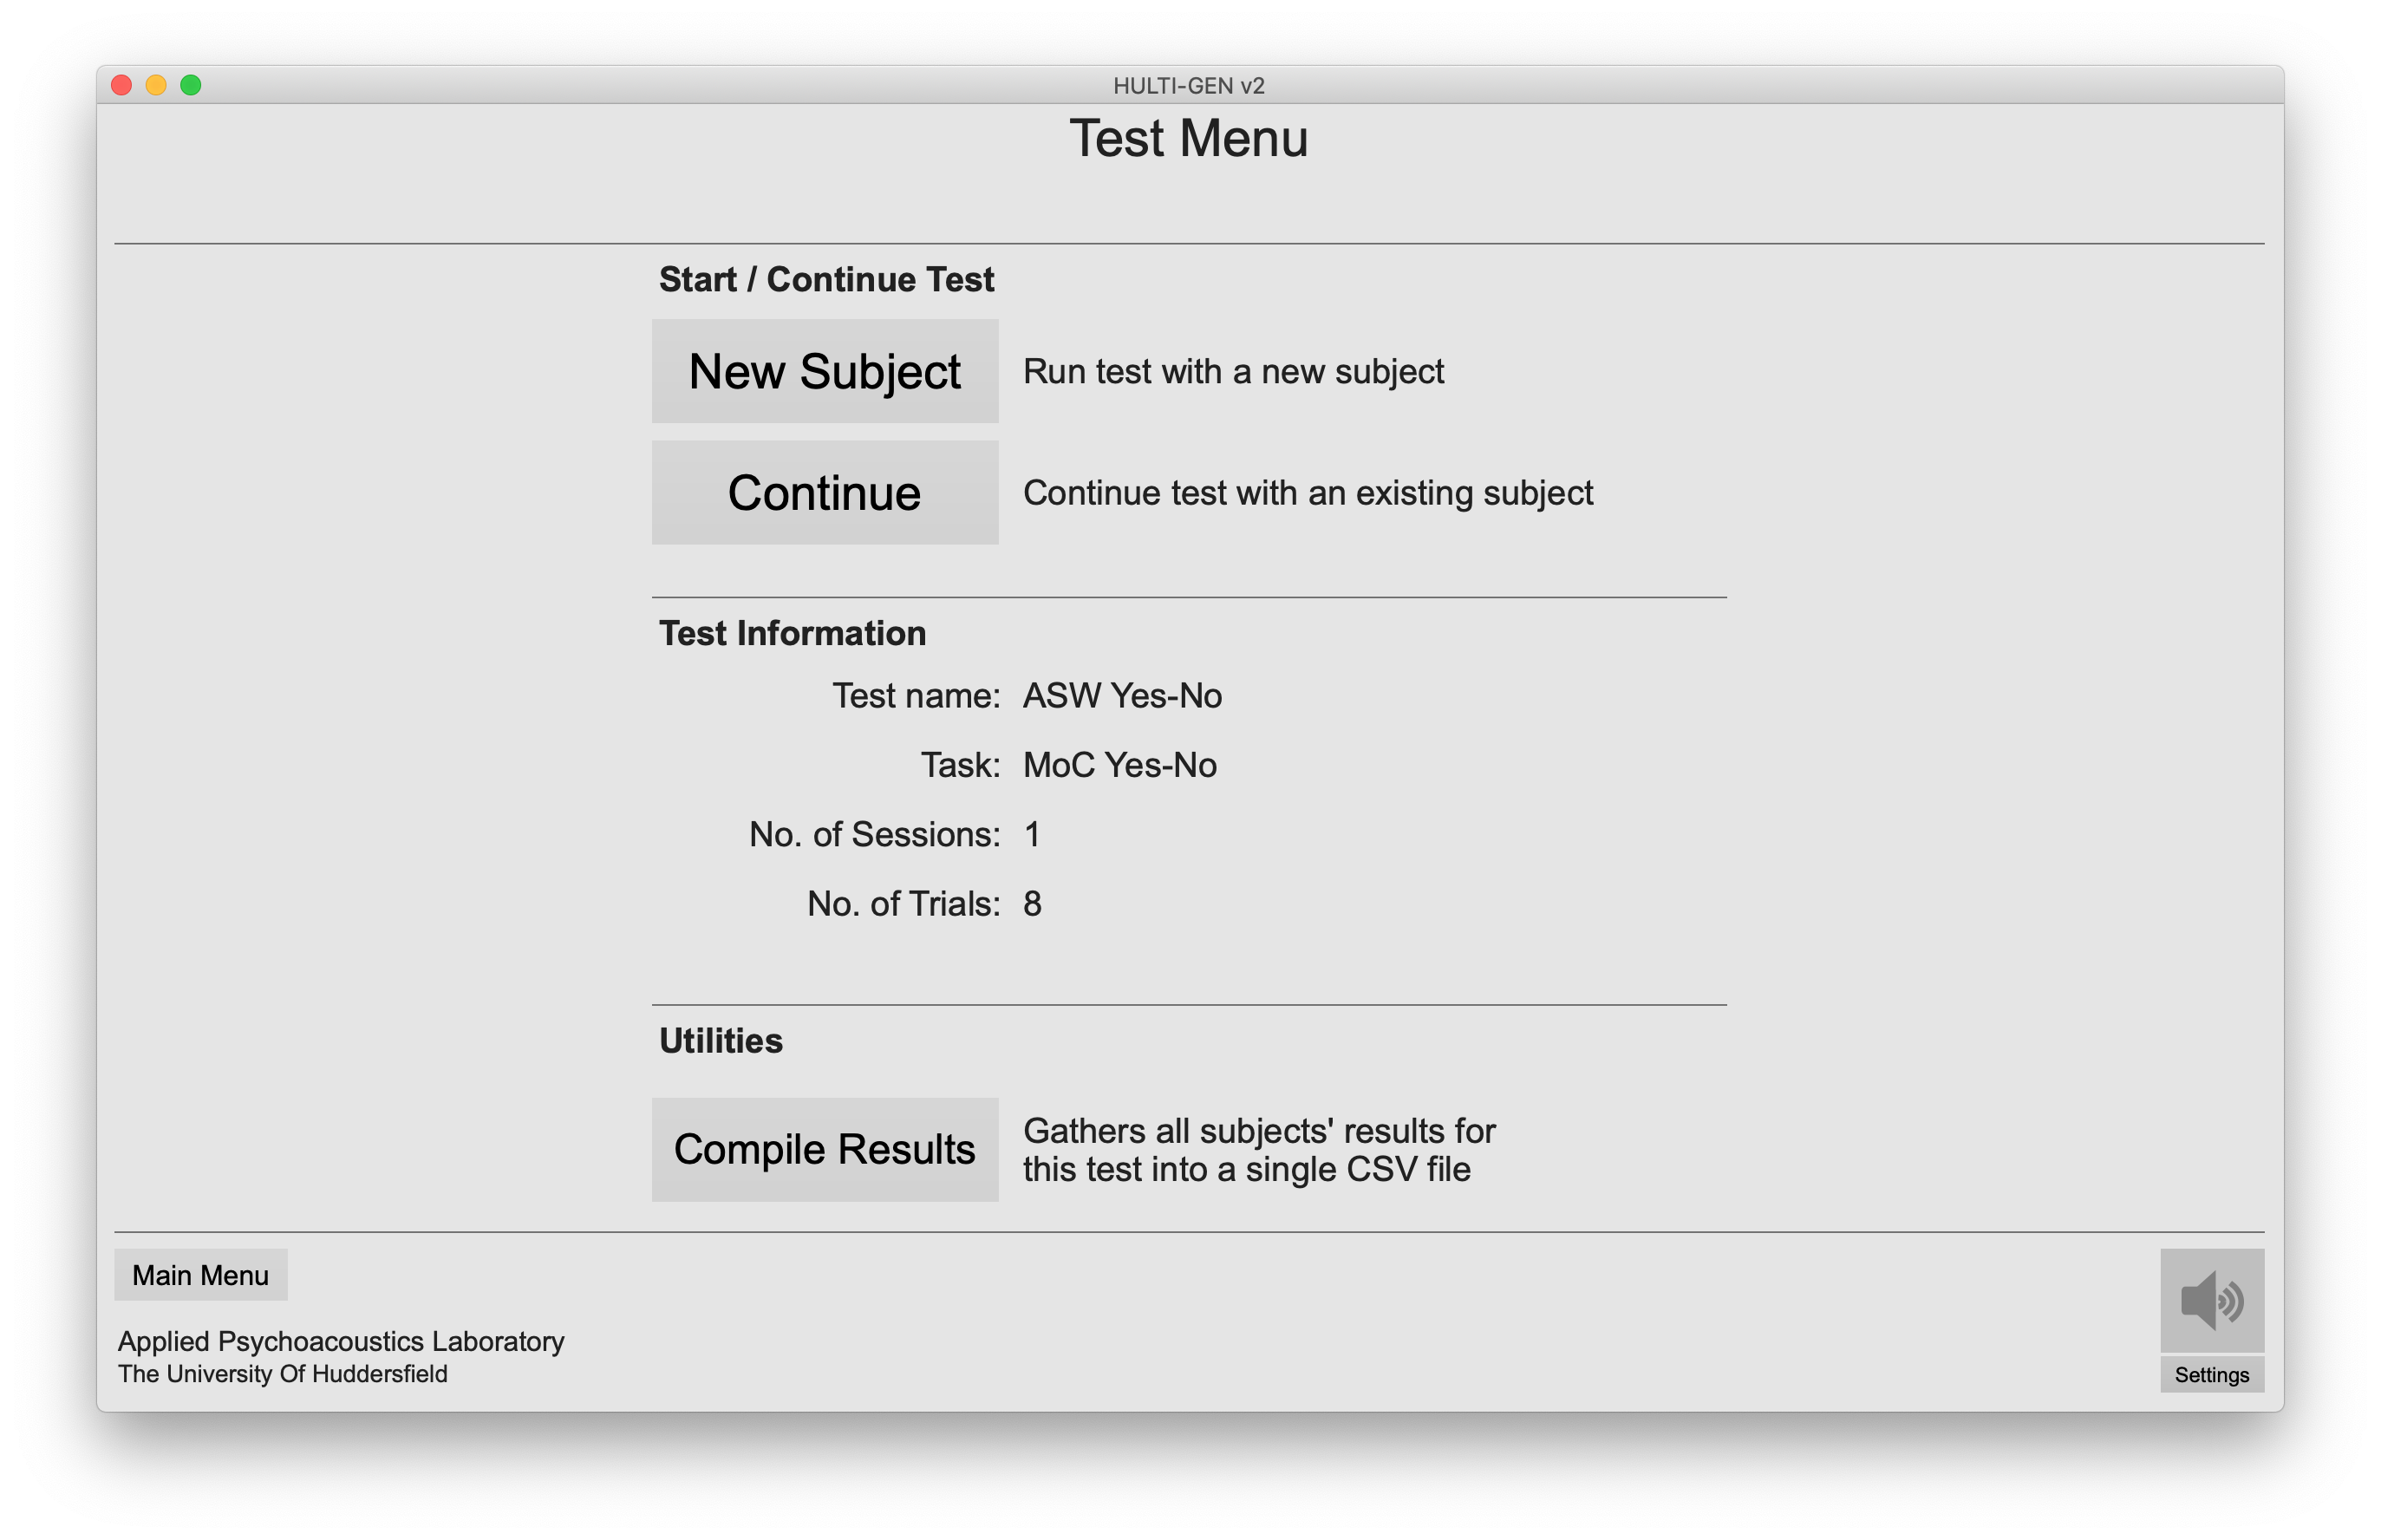
\includegraphics[width=1.0\textwidth]{./images/run_testMenu.png}
	\caption{The Test Menu, where you can choose to run the test with a new subject or continue with an existing subject.}
	\label{run::testingMenu}
\end{figure}
\pagebreak

\section{Starting with a new subject}
When you start the test with a new subject, you will be prompted to enter an identifier for this subject, and then where to save their data file. You will then be prompted to begin the test. This displays what sitting and group they are about to begin, and will give the subject a moment to compose themselves. When the subject is ready, they can press 'Begin'.
\newline\newline
\noindent
\textit{\textbf{Note:} Don't forget to turn on the audio processing, otherwise your subject will not hear anything.}

\begin{figure}[ht]
	\centering
	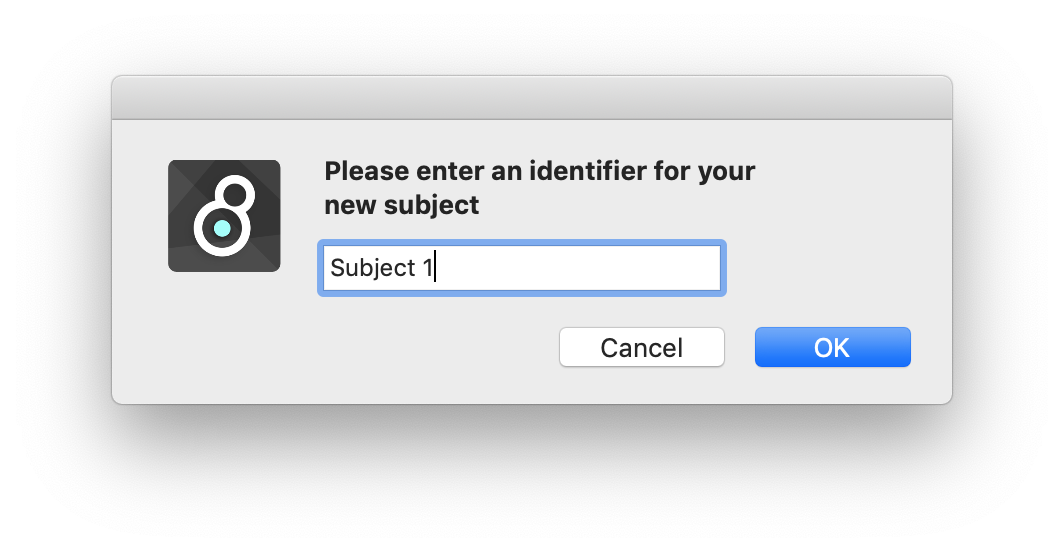
\includegraphics[width=0.6\textwidth]{./images/run_identifier.png}
	\caption{Subject identifier prompt.}
	\label{run::indentifier}
\end{figure}

\begin{figure}[ht]
	\centering
	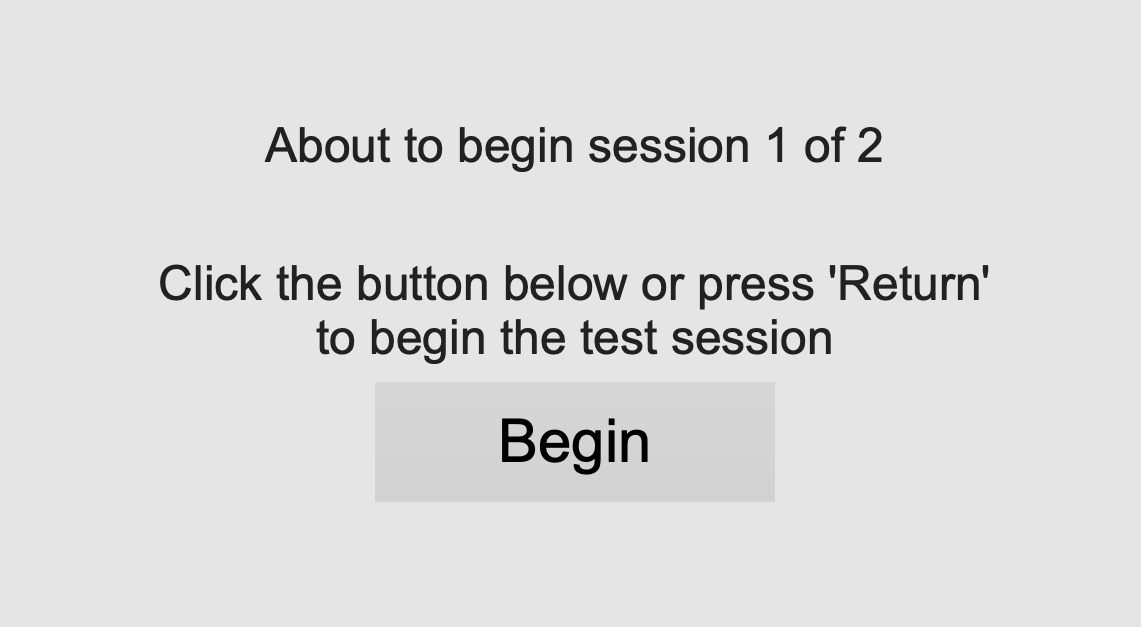
\includegraphics[width=0.5\textwidth]{./images/run_begin.png}
	\caption{The subject is informed of their progress before beginning the test.}
	\label{run::begin}
\end{figure}

\section{Test completion and results output}
The subject will carry out the test for as many trials and groups outlined by the test parameters. When they have completed all groups in a session, their data file is automatically saved, and they may leave the session. Once a subject has finished all sessions in a test, the experiment data is automatically exported as a Comma Separated Values (CSV) file, by which you will be prompted on where to save this file.